%%%%%%%%%%%%%%%%%%%%%%%%%%%%%%%%%%%%%%%%%%%%%%%%%%%%%%%%%%%%%%%%%%%%%%
% Template Source: Dave Richeson (divisbyzero.com), Dickinson College
% Author: Louis Dod (13bytes.de)
%%%%%%%%%%%%%%%%%%%%%%%%%%%%%%%%%%%%%%%%%%%%%%%%%%%%%%%%%%%%%%%%%%%%%%
% Please report any errors either via pull request, issue (https://github.com/13Bytes/Uni-Merkzettel) or mail (coding@13bytes.de)
% Improvements are also gladly accepted
%%%%%%%%%%%%%%%%%%%%%%%%%%%%%%%%%%%%%%%%%%%%%%%%%%%%%%%%%%%%%%%%%%%%%%


\documentclass[a4paper,10pt,landscape]{article}
\usepackage{fontspec}
\usepackage[T1,EU1]{fontenc}
\usepackage{lmodern}    % font
\usepackage[frenchb]{babel} 
\usepackage{amssymb,amsmath,amsthm,amsfonts}
\usepackage{multicol,multirow}
\usepackage{calc}
\usepackage{ifthen}
\usepackage{mathrsfs}
\usepackage[landscape]{geometry}
\usepackage[colorlinks=true,citecolor=blue,linkcolor=blue]{hyperref}
\usepackage[colorinlistoftodos, ngerman]{todonotes}
\usepackage{xcolor,soul}
\usepackage{cancel}
\usepackage{mathabx}
\definecolor{lime}{RGB}{51, 204, 51}
\definecolor{neptune}{RGB}{131,194,188}

\ifthenelse{\lengthtest { \paperwidth = 11in}}
    { \geometry{top=.5in,left=.5in,right=.5in,bottom=.5in} }
	{\ifthenelse{ \lengthtest{ \paperwidth = 297mm}}
		{\geometry{top=.2cm,left=1cm,right=1cm,bottom=.2cm} }
		{\geometry{top=.2cm,left=1cm,right=1cm,bottom=.2cm} }
	}
\pagestyle{empty}
\makeatletter
\renewcommand{\section}{\@startsection{section}{1}{0mm}%
                                {-1ex plus -.5ex minus -.2ex}%
                                {0.5ex plus .2ex}%x
                                {\normalfont\large\bfseries}}
\renewcommand{\subsection}{\@startsection{subsection}{2}{0mm}%
                                {-1explus -.5ex minus -.2ex}%
                                {0.5ex plus .2ex}%
                                {\normalfont\normalsize\bfseries}}
\renewcommand{\subsubsection}{\@startsection{subsubsection}{3}{0mm}%
                                {-1ex plus -.5ex minus -.2ex}%
                                {1ex plus .2ex}%
                                {\normalfont\small\bfseries}}
                                
\newcommand{\OK}{\fcolorbox{black}{lime}{\rule{0pt}{1pt}\rule{1pt}{0pt}}}
\newcommand{\NO}{\fcolorbox{black}{red}{\rule{0pt}{1pt}\rule{1pt}{0pt}}}
\DeclareRobustCommand{\hlcy}[1]{{\sethlcolor{cyan}\hl{#1}}}
\newcommand{\NDTIME}{\textrm{\textcolor{yellow}{D}\textcolor{orange}{N}TIME}}
\newcommand{\NDSPACE}{\textrm{\textcolor{yellow}{D}\textcolor{orange}{N}SPACE}}
                
\makeatother
\setcounter{secnumdepth}{0}
\setlength{\parindent}{0pt}
\setlength{\parskip}{0pt plus 0.5ex}
% -----------------------------------------------------------------------

\begin{document}

\raggedright
\footnotesize

Merkblatt Theo 2 - Matr.: \hspace{3cm} Name: \hspace{16cm}
{\tiny{\href{https://github.com/13Bytes/Uni-Merkzettel}{\textcolor{gray}{github.com/13Bytes/Uni-Merkzettel}}}}\\

\begin{multicols}{3}
    \setlength{\premulticols}{1pt}
    \setlength{\postmulticols}{1pt}
    \setlength{\multicolsep}{1pt}
    \setlength{\columnsep}{2pt}

    % -----------------------------------------------------------------------

    \section{Berechenbarkeit}
    \subsection{LOOP-Berechenbar}
    \textcolor{orange}{LOOP $x_i$ DO P END} und Zeichen \textcolor{orange}{$;$}, \textcolor{orange}{$:=$}, \textcolor{orange}{$+$}, \textcolor{orange}{$-$} (mod. Subtstrak.)

    \textcolor{orange}{$P$} wird mit initialem Wert $x_i$ oft ausgeführt.
    Alle Variablen $x_i$, $i\in \mathbb{N}$, sind mit $0$ initialisiert.
    $x_0$ ist Ausgabe. Parameter $f(x_1, x_2, ...)$ werden in Var. $x_1, x_2, ...$ geschrieben
    \hrule
    \smallskip

    \subsection{= Primitive Rek.}
    Grundfunktionen:
    \begin{itemize}
        \item $k: \mathbb{N}^l \rightarrow \mathbb{N}$ konstante Funktion
        \item $ \Pi_i^l: \mathbb{N}^l \rightarrow \mathbb{N}$ Projektion auf i-tes Element $(x_1, ..., x_l) \rightarrow x_i$
        \item $s(n) = n+1$ Nachfolger
        \item Einsetzen mit $g: \mathbb{N}^m \rightarrow \mathbb{N},\  h_i:\mathbb{N}^l \rightarrow \mathbb{N}$\\
            $\Rightarrow \mathbb{N}^l \rightarrow \mathbb{N} \ (x_1, ..., x_l) \mapsto 
            g(h_1(x_1,...,x_l), ..., h_m(x_1, ..., x_l))$
        \item Primitive Rekursion:
        $f(n, x_1, ...,x_k) = \left\{
                                    \begin{array}{ll}
                                        g(x_1, ..., x_k), & n=0 \\
                                        h(f(n-1, x_1, ..., x_n), n, x_1, ..., x_k), & sonst
                                    \end{array}
                                \right.$
        
        \textcolor{lime}{
        $g(x)=0 \quad h(z,n,x)=\text{add}(z,x) \quad \Rightarrow \ f(y,x) = y \cdot x $
        }

        \vspace{5pt}
        \textcolor{lime}{
        $\textrm{even}(0)=1=c^{0}_1 $ \\
        $\textrm{even}(x+1)=\textrm{zero}(\textrm{even}(x)) =
        \textrm{zero}(\Pi^2_1(\textrm{even}(x),x)) $
        }
    \end{itemize}
    \hrule
    \smallskip


    \subsection{$\subsetneq$ WHILE-, GOTO-Berechenbar}
    (da Ackermannfunktion oder nirgends definierte Funktion nicht LOOP-berch.)

    WHILE $x_i \neq 0$ DO $P$ END
    \hrule
    \smallskip


    \subsection{= Turing-Berechenbar}
    TM $M_i$ exisitiert für $f(n_i, ..., n_k) = m$. $M_i$ hält mit $m$ auf Ausgabe-band, wenn Eingabe das Tupel $(n_1, ..., n_k)$ war.
    \hrule
    \smallskip

    \subsection{= $\mu$-Berechenbar ($\mu$-Rekursiv)}
    mit $f: \mathbb{N}^{k+1}\rightarrow \mathbb{N} \quad \textcolor{red}{\mu f}:\mathbb{N}^k \rightarrow \mathbb{N}$ \\
    $\mu f(x_1, ..., x_k) =  \text{min}\left\{\ n \ |\ f(n, x_1, ..., x_k)=0 \ \land \
    \forall m<n:f(m, x_1, ..., x_k) > 0 \right\}$ \\
    \textcolor{lime}{Für $f(x,y)=2$ ist $\mu f$ nirgends def.} \\
    \textcolor{blue}{Sei $f$ $\mu$-Rekursiv.s
    Dann exist. $p,q$ als $(k+1)$-stellige prim. rekursive Funktionen mit:\\
    $f(x_1, ..., x_k) = p(x_1, ..., x_k, \mu q(x_1, ..., x_k))$\\
    $\sim$ Satz von Kleene \\
    $\Rightarrow$ Eine einzige While-Schleife kann das gleiche berechnen, wie ein Programm mit mehren Schleifen.
    }
    \hrule
    \smallskip

    \subsection{= Arithmetisch Repräsentierbar}
    Terme $t_1, t_2, ...$ bilden Formeln zB: $t_1=t_2$\\
    Formeln: $\neg F, F\land G, ...$. Quantoren $\exists, \forall, \in$ erzeugen gebundene Var.\\
    Belegungen mit zB $\Phi(x)=3,\ \Phi(y)=3, ... \ $ führen zu wahren/falschen Aussagen $\Phi(F)$

    $f: \mathbb{N}^k \rightarrow \mathbb{N}$ ist arithmetisch repräsentierbar, falls $F$ existiert mit:\\
    $F(n_1, ..., n_k, m) \ \Leftrightarrow \ f(n_1, ..., n_k) = m$\\
    \textcolor{lime}{$f(x,y)=x \cdot y$ a.r. mit $F(x,y,z) \Leftrightarrow ((x\cdot y)=z)$}\\
    Element: \textcolor{lime}{$x\geq 1 \ \Rightarrow \ \exists k: k+1=x $}\\
    \textcolor{gray}{Danach Korrektheit beweisen: $F$ wahr $\Leftrightarrow$ ... $=f$}
    \hrule
    \smallskip

    \subsection{Church'sche These}
    Alle diese letzten Modelle beschreiben das gleiche, wie der intuitive Berechenbarkeitsbegriff.
    \hrule
    \smallskip

    \vspace{10pt}
    \section{Wachstum}
    von Programm $P$ werden alle Var aufsummiert: \hspace{2pt} $f_p(n) = \text{max}\left\{ \sum_{i\geq 0} n_i' \ |\ \sum_{n_i \geq 0} n_i \leq n \right\}$ 

    Bei LOOP: $\exists k: \forall n: f_p(n)<a(k,n)$

    \hrule
    \smallskip

    \section{Entscheidbarkeit}
    Menge ist \textbf{Entscheidbar}, wenn für Menge $A$ charakteristische Funktion $\chi_A$ berechenbar ist. \hspace{2pt}
    $\chi_A(w) =
        \left\{
        \begin{array}{ll}
        1, & w\in A \\
        0, & w\not\in A
        \end{array} \right. $

    \textcolor{blue}{$A \text{ entscheidbar} \Leftrightarrow A, \bar{A}$ semi-entscheidbar}

    Menge ist \textbf{Semi-Entscheidbar}, wenn $\chi_A'$ wahr für $w \in A$ zurück gibt (also hält). \hspace{3pt} 
    $\chi_A(w) =
        \left\{
        \begin{array}{ll}
        1, & w\in A \\
        \text{undef.}, & w\not\in A
        \end{array} \right. $

    \textbf{Semi-Entscheidbar} ist äquivalent zu:
    \begin{itemize}
        \item  \textbf{rekursiv Aufzählbar}: $\exists f: \mathbb{N} \rightarrow \Sigma^* $ \hspace{1pt}:\hspace{1pt}  $A = \{ f(n) | n \in \mathbb{N} \}$
        \item $A$ ist Typ 0
        \item $\exists$ Turing Maschine $M$: $A=T(M)$
        \item $\chi'$ ist berechenbar
        \item A ist Definitions- oder Zielbereich von berechenbarer Funktion.
    \end{itemize}

    \subsection{Halteproblem}
    spezielles Halteproblem $K = \{ w \in \{0,1\}^* \ |\ M_w \textrm{ hält auf Eingabe } w \}$

    Halteproblem $H = \{ w\#x \  |\ M_w \textrm{ hält auf Eingabe } x \}$
    Halteproblem $H_0 = \{ w \ |\ M_w \textrm{ hält auf Eingabe } \epsilon \}$

    \subsection{\textcolor{blue}{Satz von Rice}}
    \textcolor{blue}{Nicht-triviale Aussagen über die Spracheigenschaften von TM sind unentscheidbar.}\\
    \textcolor{gray}{
    $S \subseteq R$ turing-berechenbare Funk. mit $ \emptyset \neq S \neq R$\\
    $C(s) = \{ w \ |\ M_w \textrm{ berechnet eine Funktion aus } S \}$ ist unentscheidbare Menge.
    }\\
    \textcolor{red}{Nur für Sprachen verwenden, deren Elemente kodierte TMs sind!}\\
    \textbf{Verwendung im Beweis}: \\
    - Zeigen: Sprache ist semantisch (z.B: Hängt nur von $T(M)$ ab)\\
    % \todo[inline]{Sprache ist semantisch ausführen}
    - Zeigen: Sprache ist nicht trivial. (Beispiele von Eingaben, für die Sprache jeweils wahr/falsch)






    \hrule
    \smallskip



    \section{Komplexität}
    Alle deterministischen Klassen sind gegen Komplement abgeschlossen.

    \textcolor{lime}{zB: $A \in \textrm{DTIME}(\mathcal{O}(\log (n)))$}
    \subsection{Zeitklassen}
    DTIME ist gegen Komplement abgeschlossen\\
    NTIME nicht.
    \subsubsection{P - \textit{Polynomialzeit}}
    durch LOOP-Programme entscheidbar

    \subsubsection{NP - \textit{Nichtdeterministische Polynomialzeit}}
    \textbf{NP-hart} $\forall L \in \textrm{NP}: \ L \leq_p A$ \\
    \textbf{NP-vollständig} NP-hart und Sprache $A \in \textrm{NP}$

    \textcolor{blue}{$A \leq_p B \ \land \ B\in \textrm{(N)P} \Rightarrow A \in \textrm{(N)P}$}\\
    \textcolor{gray}{
    Beweis $A \in$ NP oft mit guess \& check
    }

    \subsubsection{EXPTIME - \textit{Exponentialzeit}}
    $2^{p(n)}$ mit Polynom $p$


    \subsection{Platzklassen}
    SPACE und NSPACE sind gegen Komplement abgeschlossen,\\
    wenn $f\in \Omega(\log(n))$ \hspace{10pt}
    $\Rightarrow \ \textrm{NSPACE}(f) = \textrm{coNSPACE}(f)$

    \vspace*{5pt}
    Wird $x$ viel Platz nicht verlassen, endet die Maschine nach spätestens $|x| \cdot |Z| \cdot |\Gamma|^{(|x|+1)} $ in einer Schleife

    \subsubsection{L = LOGSPACE - \textit{logarithmischer Platz}}

    \subsubsection{NL - \textit{nichtdeterministischer log. Platz}}

    \subsubsection{PSPACE - \textit{polynomieller Platz}}
    \textcolor{gray}{
    $=\bigcup_{k\geq 1}\textrm{DSPACE}(n^k) = \bigcup_{k\geq 1}\textrm{NSPACE}(n^k)$
    }

    \hrule
    \smallskip

    \subsection{Zeit- / Platzrelationen}
    \textcolor{blue}{
    $\textrm{DTIME}(f)\subseteq \textrm{DTIME}_{2-\textrm{Band}}(f \log f)$\\
    $\sim$ Satz von Hennie und Stearns
    }
    (wenn $\epsilon > 0$ mit $\forall n:f(n) \geq (1+\epsilon)n$ existiert)\\

    \vspace*{5pt}
    $\textrm{\NDSPACE}(f) = \textrm{\NDSPACE}_{1-\textrm{Band}}(f)$\\

    \vspace*{7pt}
    \textcolor{blue}{
    $\textrm{DTIME}(f) = \textrm{DTIME}(\mathcal{O}(f)) \ $} 
    falls $ \exists \epsilon > 0: \forall n:\ f(n)\geq (1+\epsilon)n$ \\
    \textcolor{blue}{
    $\textrm{NTIME}(f) = \textrm{NTIME}(\mathcal{O}(f)) \ $} immer \\
    \textcolor{blue}{
    $\sim$ Zeit-/Platz-kompressionssatz
    }

    \vspace*{7pt}
    \textcolor{blue}{$\textrm{DTIME}(f)\subseteq  \textrm{NTIME}(f) \subseteq \textrm{DSPACE}(f)$ }
    $\forall f: \mathbb{N}\rightarrow \mathbb{N}, \forall n: f(n)\geq n$\\
    \textcolor{blue}{$\textrm{DSPACE}(f)\subseteq  \textrm{NSPACE}(f) \subseteq \textrm{DTIME}(2^{\mathcal{O}(f)})$ }
    $\forall  f: \mathbb{N}\rightarrow \mathbb{N},$\\$\ \forall n: f(n)\geq \log(n)$ - exponentieller Blowup\\
    \textcolor{blue}{$\Rightarrow \textrm{DSPACE}(f)\subseteq \textrm{DTIME}(2^{\mathcal{O}(f)})$}

    \vspace*{7pt}
    \textcolor{blue}{
    $\textrm{NSPACE}(s)\subseteq \textrm{DSPACE}(s^2)$} mit $s \in \Omega(\log n)$\\
    \textcolor{blue}{$\sim$ \textbf{Satz von Savitch}\\
    }

    \subsection{Zeit- / Platzkonstruierbar}
    Deterministische TM existiert, die bei unär kodierter Eingabe $a^n$ der Länge $n$, $f(n)$ viel Platz/Zeit braucht.

    \hrule
    \smallskip

    \subsection{\_\_\_-Hierarchiesatz}
    \textbf{Platz:} Sei
    $s_1, s_2: \mathbb{N} \rightarrow \mathbb{N} \ ,\
    s_1 \notin \Omega(s_2) \ ,\ s_2\in\Omega(\log n) \ ,\  s_2$~platzkonstruierbar \\
    \textcolor{blue}{ $\textrm{DSPACE}(s_2) \backslash \textrm{DSPACE}(s_1) \neq \emptyset$}\\
    Beweis für $s_1\notin \Omega(s_2): \quad \forall c>0: \exists a\in \mathbb{N}: s_1(a) < c\cdot s_2(b)$
    Aufstellen und $a$ suchen, für das Gleichung stimmt.\\
    \textcolor{lime}{$ \Rightarrow \quad \textrm{DSPACE}(\log) \subsetneq \textrm{DSPACE}(\log^2)$}

    \vspace*{8pt}
    \textbf{Zeit:} Sei
    $t_1, t_2: \mathbb{N} \rightarrow \mathbb{N} \ ,\
    t_1 \log(t_1) \notin \Omega(t_2) \ ,\ t_2\in\Omega(n \log(n)) \ ,\  t_2$~zeitkonstruierbar \\
    \textcolor{blue}{ $\textrm{DTIME}(t_2) \backslash \textrm{DTIME}(t_1) \neq \emptyset$}\\
    \textcolor{lime}{$ \Rightarrow \quad \textrm{DTIME}(\mathcal{O}(n)) \subsetneq \textrm{DTIME}(\mathcal{O}(n^2))$}

    \vspace*{8pt}
    \textcolor{blue}{ 
    Sei $r$ total und berechenbar. $\forall n: r(n)\geq n$ \\
    $ \Rightarrow \exists$ totale Funktion $ s: \mathbb{N} \rightarrow  \mathbb{N} \quad s(n) \geq n+1 \ $
    mit $\textrm{DTIME}(s) = \textrm{DTIME}(r \circ s)$ \\
    $\sim $ Satz von Borodim\\
    }
    ($s$ ist nicht zeitkonstruierbar)
    % \hrule
    % \smallskip


    \newpage
    \section{Probleme}
    \hl{Zeit}, \hlcy{Platz}

    \subsubsection{PCP - \textit{Post-Korrespondenz-Problem}}
    $\chi_{\textrm{PCP}}$ ist berechenbar $\Rightarrow$ PCP ist rek. aufzählbar. $\Leftrightarrow$ semi-entscheidbar.\\
    PCP ist aber unentscheidbar (für $\Sigma \geq 2$)
    \textcolor{gray}{$\textrm{H}\leq \textrm{MPCP}\leq\textrm{PCP}$}


    \subsubsection{SAT - \textit{Satisfiablity}}
    \hl{NP-vollständig}\\
    SAT $=\{ \textrm{F} \ |\ \textrm{F ist erfüllbar} \}$\\
    \textcolor{gray}{Algos aktuell bei $2^{c\cdot n}$ (also $\in$ E)}\\
    Allgemein äquivalent zu\\
    \textbf{3KNF-SAT}, beide \hl{NP-vollständig}\\
    \textbf{2KNF-SAT} $\in$ P \& \hlcy{NL-vollständig}


    \subsubsection{CLIQUE}
    \hl{NP-vollständig}\\
    Graph $G = (V,E), \quad k\in\mathbb{N}$\\
    $V' \subseteq V$ ist Clique, falls $\forall u,v \in V': \ u\neq v \ \Rightarrow \ (u,v) \in E$

    CLIQUE $\in$ NP durch guess \& check.\\
    NP-Vollständigkeit durch 3KNF$\cdot$SAT$\leq$CLIQUE
    mittels Graph mit $E=\{\{(r,s),(p,q)\} | r\neq p \land z_{rs}\not\equiv \neg z_{pq} \}$
    (Alle Literale, die sich nicht gegenseitig ausschließen)


    \subsubsection{FÄRBBARKEIT}
    \hl{NP-vollständig}\\
    $\varphi:V\rightarrow\{1,...,k\}$ für Graph $G = (V,E), \quad k\in\mathbb{N}$,\\
    Knotenfärbung mit $k$ Farben: $\forall(u,v)\in E:\ \varphi(u)\neq \varphi(v)$

    FÄRBBARKEIT $\in$ NP durch guess \& check.\\
    NP-Vollständigkeit durch 3KNF$\leq$3-Färbbarkeit


    \subsubsection{GAP - \textit{Grapherreichbarkeit}}
    \hlcy{NL-vollständig}\\
    Auf Graph $G = (V,E), \quad k\in\mathbb{N}$ und 2 Knoten: $s,t\in V$\\
    Kann man über Kanten $\in E$ von $s$ zu $t$ gelangen?\\
    \textcolor{gray}{DSPACE($\log^2n$)}\\

    GAP $\in$ NP, da:\\
    WHILE $ v\neq t$ DO \{ \\
    Wähle nicht-det. $w\in V$, \hspace{3pt} aus $(v,w)\in E$\\
    $v=w$ \}\\
    RETURN 1


    \subsubsection{CVP - \textit{Circuit Value Problem}}
    \hl{P-vollständig}
    Bei Schaltkreisen können (Teil)formeln wiederverwendet werden.


    \subsubsection{QBF - \textit{Quantifizierbare Boolsche Formeln}}
    \hlcy{PSPACE-vollständig}


    \subsubsection{TSP - \textit{Traveling Salesman Problem}}
    \hl{$\in$NP}


    \subsubsection{VC - \textit{Vertex Cover}}


    \hrule
    % \smallskip
    \columnbreak

    \vspace{5pt}
    \section{Allgemeines}
    TM $M=(Z,\Sigma,\Gamma, \delta, z,  \square ,E)$ - Z: Zustandsmenge, $\Gamma$: Bandalphabet,\\
    Übertragungsfunktion $\delta(z_i,a)= (z_j, a',\textrm{L})$, z: Startzustand\\
    $a, a' \in \Gamma$, statt L auch L,R,N\\
    Sprache T(M)\\
    \textcolor{gray}{TM ist äquivalent zu Mehrband-TMs und nicht det. TM}

    \vspace{3pt}
    Grammatik: $G=(V,\Sigma, P,S)$ mit $P\subseteq(V\cup\Sigma)^+ \times (V\cup\Sigma)^*$

    \vspace{3pt}
    Disjunktion: $\lor$, Konjunktion $\land$,
    DNF: $ \bigvee_i \bigwedge_j (\neg)x_{ij} $\\
    Bestimmte Verknüpfung der Unterterme.\\

    $\dotdiv$ Modifizierte Differenz: $ \max\{0,a-b\}=\textrm{md}(a,b)$

    Belegung $\mathscr{A}$ passt zu Formel F, wenn jede vorkommende atomare Variable einen Wert zugewiesen bekommt.\\
    Belegung $\mathscr{A}$ ist Modell, wenn passend und $\mathscr{A}(F) = 1$.\\
    Formel F ist gültig, wenn für alle $\mathscr{A}$, die zu F passen, $\mathscr{A}(F) = 1$ gilt (Tautologie).
    \textcolor{gray}{''Ungültig'' existiert nicht}

    $\binom{n}{k} = \dfrac{n!}{(n-k)! \cdot k}$

    Nirgends definierte Funktion $\Sigma$ (berechenbar)

    \hrule
    \smallskip

    \subsection{Ackermann-Funktion $\textrm{A}(n)= \textrm{a}(n,m)$}
    \arraycolsep=1.4pt
    $\begin{array}{ll}
    \textrm{a}(0,y) &= y+1 \\
    \textrm{a}(x,0) &= \textrm{a}(x-1,1)\\
    \textrm{a}(x,y) &= \textrm{a}(x-1,\textrm{a}(x,y-1))
    \end{array}$
    \textcolor{gray}{$x,y>0$}\\
    \vspace{2pt}
    \textcolor{lime}{
    $\begin{array}{ll}
    y &< \textrm{a}(x,y) \\
    \textrm{a}(x,y) &< \textrm{a}(x,y+1) \\
    \textrm{a}(x,y+1) &\leq \textrm{a}(x+1,y) \\
    \textrm{a}(x,y) &< \textrm{a}(x+1,1)\\
    \end{array}
    $}
    \hrule
    \smallskip

    \subsection{Bijektion $\mathbb{N}^2 \rightarrow \mathbb{N}$}
    Kodieren von Tupeln:\\
    $\textrm{c}(x,y)= \binom{x+y+1}{2}+x$
    $=\textrm{add}(f(s(\textrm{add}(x,y))),x)$

    \subsection{Dove-Tailing}
    \begin{itemize}
        \item $\Sigma^* =\{w_1, w_2, ...\}$ Längenlexikographisch Anordnen
        \item 
        FOR $i=0,1,2, ...$ DO\\
        \hspace*{7pt}Simuliere $i$ Schritte von $M_w$ auf Eingabe $e(i)$\\
        \hspace*{7pt}...Kriterium...
    \end{itemize}
    \hrule
    \smallskip


    \subsection{Translationstechnik}
    Padding einer Sprache mit $\$ \notin \Sigma$\\
    $\textrm{Pad}_f(L) = \left\{ w \$^{f(|w|)-|w|} \ |\ w\in L \right\}$

    \textbf{Zeit}: \textcolor{blue}{
    $\textrm{Pad}_f(L) \in \NDTIME(\mathcal{O}(g)) \Leftrightarrow \textrm{L} \in \NDTIME(\mathcal{O}(g\circ f)) $}\\
    mit $f,g$ zeitkonstruierbar, $g(n),f(n)\geq n$

    \textbf{Platz}: \textcolor{blue}{
    $\textrm{Pad}_f(L) \in \NDSPACE(\mathcal{O}(g)) \Leftrightarrow \textrm{L} \in \NDSPACE(\mathcal{O}(g\circ f)) $}\\
    mit $g\in \Omega(\log)$, $\forall n: f(n)\geq n$ berechenbar

    \vspace{5pt}
    $\Rightarrow$ \textcolor{blue}{ $\textrm{DSPACE}(n)\neq \textrm{P} $}
    \hrule
    \smallskip


    \subsection{Aufzählbar / Abzählbar}
    \begin{tabular}{|c|c|}
    \hline
    \textbf{rekursiv Aufzählbar} & \textbf{Abzählbar}    \\ \hline
    \multicolumn{2}{|c|}{totale Funktion $f:\mathbb{N}\rightarrow\Sigma^*$} \\ \hline
    $f$ berechenbar          &  \\ \hline        
    \end{tabular}\\
    Mit $A\subseteq B$ folgt NICHT:\\
    $B$ rekursiv aufzählbar $\not \Rightarrow A$ rek. aufzählbar. Nur $A$ abzählbar

    \vspace*{1pt}
    \hrule
    \smallskip


    \subsection{Reduktion}
    $A$ ist auf $B$ reduzierbar $A \leq B$, wenn totale \& berechenbare Funktion $f: \Sigma^*\rightarrow\Gamma^*$ existiert mit: \\
    $x\in A \Leftrightarrow f(x) \in B$

    $\leq$ unbeschränkt \hspace{7pt}
    $\leq_p$ polynomialzeit \hspace{7pt}
    $\leq_{log}$ Logspace ($f$ ist logspace-berechenbar)

    \hspace{5pt}
    \textcolor{blue}{$A\leq B$ und B (semi-)entscheidbar $\Rightarrow$ A (semi-)entscheidbar}
    \hrule
    \smallskip


    \subsection{Landau-Symbole}
    $f\in \mathcal{O}$: f wächst nicht wesentlich schneller als ... \\
    $f\in \Omega$: f wächst nicht wesentlich langsamer als ...\\
    Beweis $f(n) \in \mathcal{O}(b(n))$: $\exists c \exists n_0 \ \forall (n \geq n_0): \ b(n) \leq c \cdot f(n) $
    \hrule
    \smallskip


    \subsection{Relationen}
    \newcommand*\rot{\rotatebox{90}}
    \begin{tabular}{|l|llllllllll|}
    \hline
        & \rot{$L_1=L_2$}
        & \rot{$L_1 \subseteq L_2$}
        & \rot{$L_1 \cap L_2 = \emptyset$}
        & \rot{$ |L_1 \cap L_2| < \infty $}
        & \rot{\begin{tabular}[c]{@{}l@{}}$ L(G) = L_1 \cap L_2 $\\ G ist Typ-2\end{tabular}}

        & \rot{Schnitt $\cap$}
        & \rot{Verein. $\cup$}
        & \rot{Kompl.}
        & \rot{Produkt}
        & \rot{Stern}
        \\ \hline
    Typ-3 Reg               &   &   &\OK&   &   & \OK  & \OK  & \OK   & \OK      & \OK    \\\hline
    DCFL                    &\OK&\NO&\NO&\NO&\NO& \NO  & \NO  & \OK   & \NO      & \NO    \\
    Det. Kntx-frei          &   &   &   &   &   &      &      &       &          &        \\\hline
    Typ-2 CFL               &\NO&\NO&\NO&\NO&\NO& \NO  & \OK  & \NO   & \OK      & \OK    \\
    Kntx-frei               &   &   &   &   &   &      &      &       &          &        \\\hline
    Typ-1 CSL               &   &   &   &   &   & \OK  & \OK  & \OK   & \OK      & \OK    \\\hline
    Typ-0                   &   &   &   &   &   & \OK  & \OK  & \NO   & \OK      & \OK    \\\hline
    \end{tabular}\\
    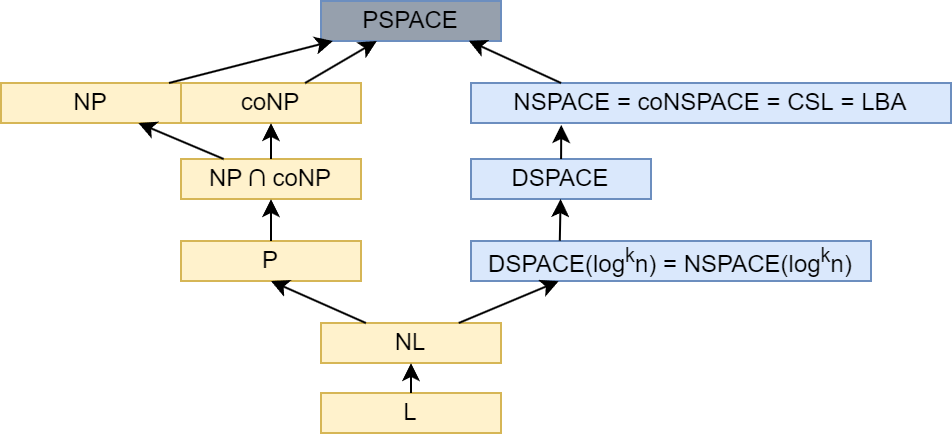
\includegraphics[width=0.26\textwidth]{Beziehungen.png}

    $\textrm{L} \subseteq
    \textrm{NL} \subseteq 
    \textrm{P}\subseteq 
    \textrm{PSPACE}\subseteq
    \textrm{EXPTIME} $
    \textcolor{lime}{
    $\Rightarrow \textrm{DSPACE}(\log n)
    \subseteq\textrm{NSPACE}(\log n)
    \subseteq\textrm{DTIME}(2^{\mathcal{O}(\log n)})
    = \textrm{P} $
    }

    \hrule
    \smallskip


    \subsection{$G(a,b,i,\cdot)$-Prädikat}
    $G(a,b,i,y) \Leftrightarrow y=a \mod (1+(i+1)\cdot b)$\\
    \textcolor{gray}{$\Rightarrow \ y\leq(i+1)b \quad (1+(i+1)b \ \% \ (a-y))=0 $}\\
    $a,b$ zwei Werte, die endliche Folge $(n_0, ..., n_k)$ kodieren.\\
    $i$ Index, $y$ Wert. Es gilt für alle $i\leq k$:\\
    $n_i = y \ \Leftrightarrow \ G(a,b,i,y)$

    \textcolor{blue}{
    $\forall k \forall (n_0, ..., n_k)\in \mathbb{N}^{k+1} \ \exists a,b \in \mathbb{N}$
    $\forall i \in \{ 0, ..., k \}: \; G(a,b,i, n_i)$
    }
    \hrule

\end{multicols}
\end{document}
